%
% 33-integralsatz.tex -- Integralsatz für allgemein Wege
%
% (c) 2026 Prof Dr Andreas Müller
%
\subsection{Integralsatz für allgemeine Wege}
Der Integralsatz~\ref{buch:integration:satz:residuensatz} beruhte darauf,
dass der Weg $\gamma$ um den Punkt sich in einen Weg deformieren liess,
der sich entlang eines Kreises genau einmal im Gegenuhrzeigersinn um den
Punkt $z_0$ windet.
Die Umlaufzahl andererseits zeigt, dass sich Wege, die sich mehrmals
um den Punkt winden, ebenfalls deformieren lassen in einen Weg, der sich
entlang einer Kreislinie mit gleichmässig ansteigendem Argument gleichviele
Male um $z_0$ windet.

\begin{satz}
\label{buch:integration:satz:residuensatzn}
\index{Satz!Cauchy-Integralsatz (Umlaufzahl)}%
\index{Cauchy-Integralsatz (Umlaufzahl)}%
Sei $f\colon U \to \mathbb{C}$ eine holomorphe Funktion und $\gamma$
ein Weg in $U$, der den Punkt $z_0$ nicht trifft, aber in den Punkt $z_0$
zusammengezogen werden kann.
Dann gilt
\[
f(z_0)
\cdot
\operatorname{ind}_{\gamma}(z_0)
=
\frac{1}{2\pi i}
\oint_\gamma \frac{f(z)}{z-z_0}\,dz.
\]
\end{satz}

Die im Satz zusätzlich geforderte Bedingung, dass der Weg in den Punkt 
$z_0$ zusammengezogen werden kann, stellt sicher, dass sich der Weg nicht
um andere ``Löcher'' im Definitionsgebiet $U$ windet, in denen sich weitere
Polstellen der Funktion $f(z)$ verstecken könnten.
%
% fig-lochgebiet.tex
%
% (c) 2026 Prof Dr Andreas Müller
%
\begin{figure}
\centering
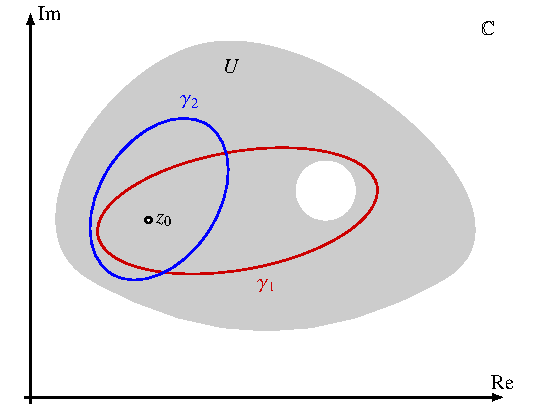
\includegraphics{chapters/030-integration/images/lochgebiet.pdf}
\caption{Zwei Wege um den Punkte $z_0$ im Gebiet $U$.
Der Weg $\gamma_1$ führt um das Loch im Gebiet $U$ herum und lässt
sich daher nicht in den Punkt $z_0$ zusammenziehen.
Dies Art von Weg kann im Satz~\ref{buch:integration:satz:residuensatzn}
nicht verwendet werden.
Nur Wege wie $\gamma_2$ sind zulässig.
\label{buch:integration:fig:lochgebiet}}
\end{figure}
%
Sie ist in Abbildung~\ref{buch:integration:fig:lochgebiet} illustriert.
Der Weg $\gamma_1$ windet sich um das Loch im Gebiet $U$ herum und kann
daher nicht in einen Punkt zusammengezogen werden, dies ist nur für den
Weg $\gamma_2$ möglich.
